\documentclass[11pt,aspectratio=169]{beamer}

\usepackage[utf8]{inputenc}
\usepackage[T1]{fontenc}
\usepackage[french]{babel}
\frenchsetup{AutoSpacePunctuation=false}
\usepackage{lmodern}
\usepackage{amsmath,amssymb,bm}
\usepackage{graphicx}
\usepackage{booktabs}
\usepackage{xcolor}
\usepackage{colortbl}
\usepackage{tikz}

%--- Theme & couleurs (bleu IMFT) --------------------------------------------
\usetheme{Madrid}
\definecolor{imftblue}{RGB}{31,73,125}
\definecolor{imftlight}{RGB}{79,129,189}
\definecolor{warnred}{RGB}{170,30,30}
\definecolor{okgreen}{RGB}{34,120,60}
\usecolortheme[named=imftblue]{structure}
\setbeamercolor{palette primary}{bg=imftblue,fg=white}
\setbeamercolor{palette secondary}{bg=imftlight,fg=white}
\setbeamercolor{palette tertiary}{bg=imftblue,fg=white}
\setbeamercolor{title}{fg=white}
\setbeamercolor{frametitle}{fg=white}
\setbeamertemplate{navigation symbols}{}
\setbeamertemplate{caption}[numbered]
\setbeamerfont{frametitle}{series=\bfseries}
\setbeamertemplate{itemize item}{\color{imftlight}\textbullet}
\setbeamertemplate{itemize subitem}{\color{imftlight}--}

\graphicspath{{sections/images/}}

%--- Page de titre ------------------------------------------------------------
\title[Ascension d'une bulle en turbulence]{Effet de la turbulence sur la vitesse d'ascension d'une bulle}
\subtitle{Simulation numérique directe (Basilisk) en turbulence homogène isotrope}
\author[Carl Bonjean Fraser]{Carl Bonjean Fraser}
\institute[ENSEEIHT / IMFT]{%
  ENSEEIHT -- Toulouse INP \quad\textbar\quad Institut de Mécanique des Fluides de Toulouse (IMFT)\\[2pt]
  \footnotesize Tuteurs de stage : Dominique LEGENDRE \& Rémi ZAMANSKY}
\date{Juillet 2026 \quad\textbar\quad Présentation des résultats du rapport}

\titlegraphic{%
  
\includegraphics[height=0.9cm]{logo_enseeiht.png}\hspace{1.2cm}%
  
\includegraphics[height=0.9cm]{logo_imft.png}}

%==============================================================================
\begin{document}

% 1. Page de titre
\begin{frame}[plain]
  \titlepage
\end{frame}

% 2. Contexte & Objectif
\begin{frame}{Contexte et Objectif Physique}
  \begin{columns}[T]
    \begin{column}{0.58\textwidth}
      \begin{block}{Question scientifique centrale}
        \textbf{La turbulence ambiante accélère-t-elle ou ralentit-elle la vitesse d'ascension d'une bulle de gaz ?}
      \end{block}

      \vspace{0.2cm}
      \textbf{Paramètres adimensionnels du cas d'étude :}
      \begin{itemize}
        \item Rapport de masse volumique : $\rho_l/\rho_g = 850$
        \item Nombre de Bond : $Bo = \frac{\rho_l g D^2}{\sigma} = 1$
        \item Nombre de Galilée : $Ga = \frac{\sqrt{gD}D}{\nu} = 70$ ($Ga > Ga_c \approx 44$, régime de trajectoire oblique)
        \item Intensité turbulente relative : $\beta = u'/u_\infty$
      \end{itemize}
    \end{column}
    \begin{column}{0.38\textwidth}
      \centering
      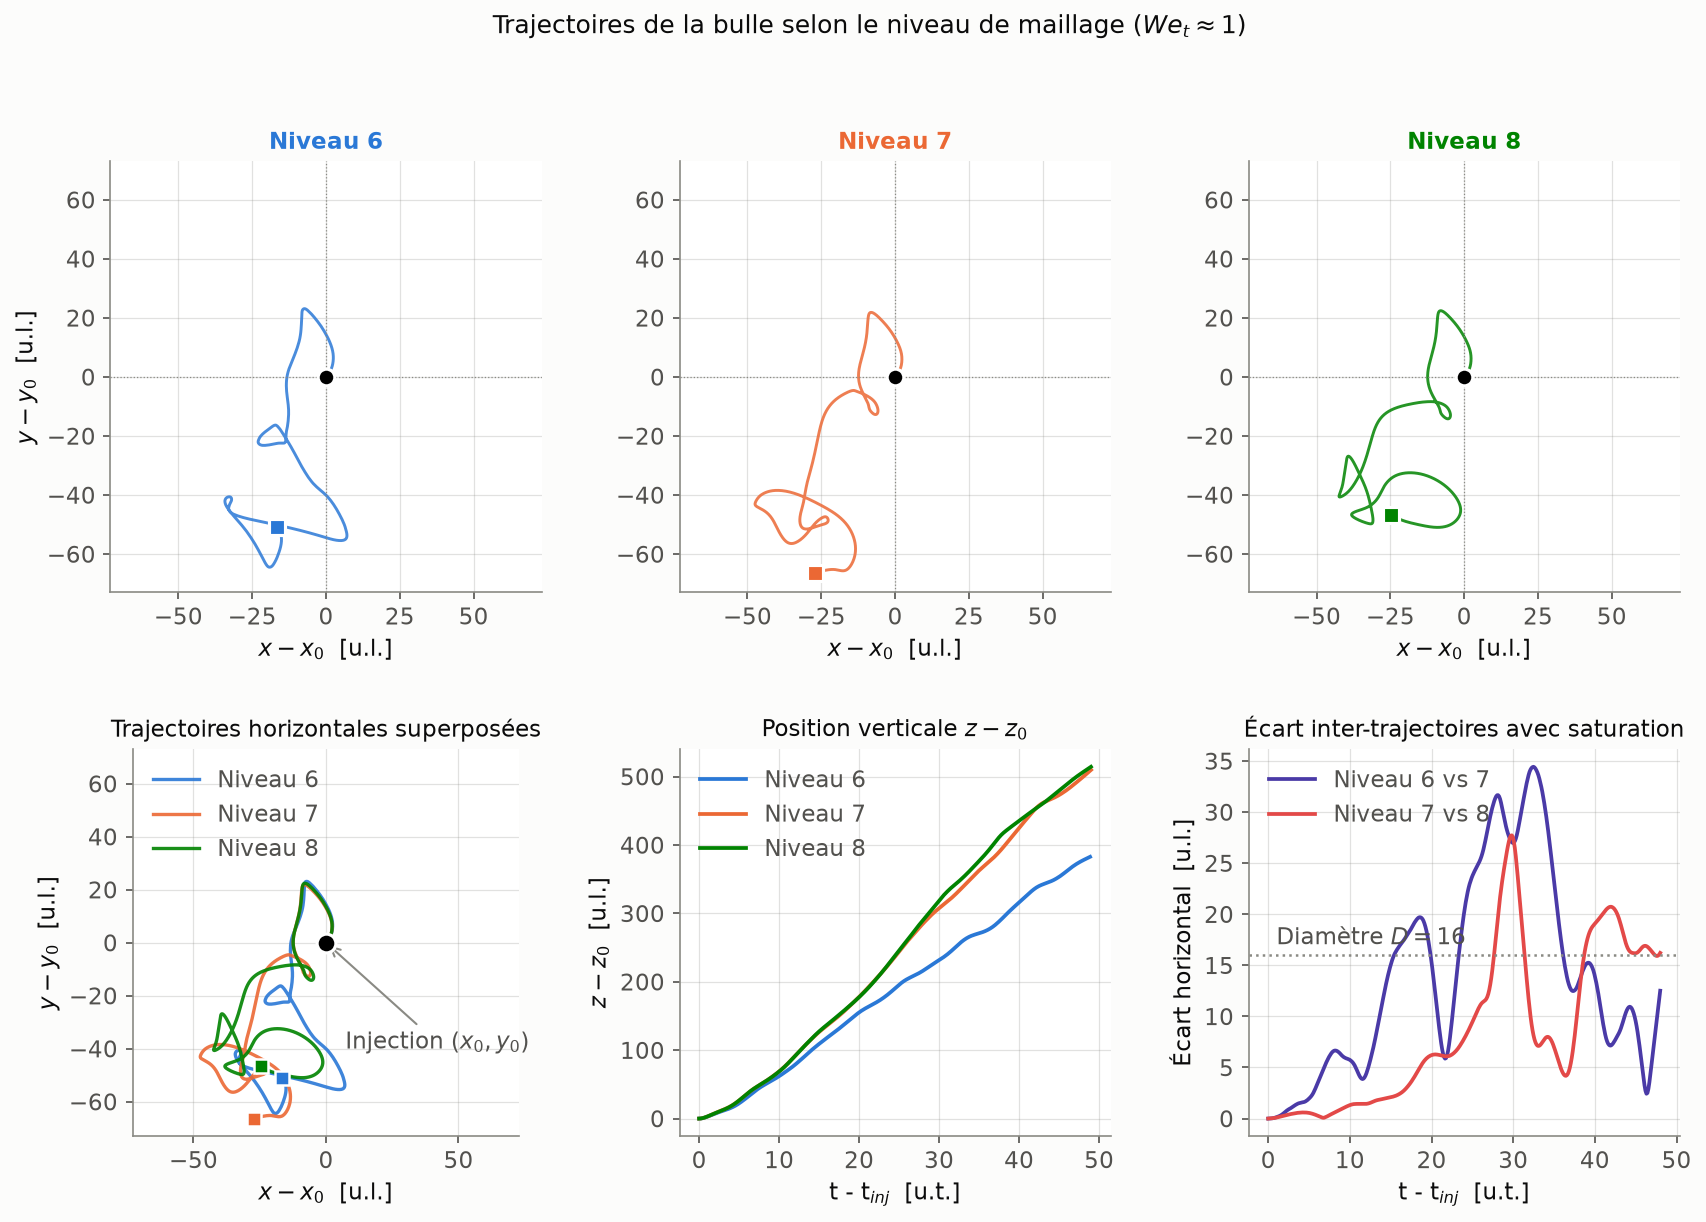
\includegraphics[width=\textwidth]{trajectoires_cote_a_cote.png}\\[2pt]
      {\scriptsize Décorrélation des trajectoires $Ga=70$}
    \end{column}
  \end{columns}
\end{frame}

% 3. Chaîne numérique & Validation
\begin{frame}{Méthode Numérique et Chaîne de Validation}
  \begin{columns}[T]
    \begin{column}{0.5\textwidth}
      \begin{block}{Solveur Basilisk (DNS / VOF)}
        \begin{itemize}
          \item Repère mobile (\texttt{event move\_frame})
          \item Maillage adaptatif octree (AMR)
          \item Modèle précurseur pour la turbulence (HIT)
        \end{itemize}
      \end{block}

      \begin{alertblock}{Validation de la chaîne numérique}
        Tous les garde-fous sont quantifiés et validés (\textbf{PASS}) :
      \end{alertblock}
    \end{column}

    \begin{column}{0.48\textwidth}
      \small
      \begin{table}
        \centering
        \renewcommand{\arraystretch}{1.2}
        \begin{tabular}{lc}
          \toprule
          \textbf{Critère de validation} & \textbf{Résultat} \\
          \midrule
          $u_\infty$ laminaire réf. & $12{,}27$ ($0{,}32\%$ dev. lvl7-8) \\
          Courants parasites & $< 0{,}08\%$ de $u_\infty$ \\
          Biais de sillage & $-0{,}8\%$ (borné) \\
          Conservation volume & $> 99\%$ tout au long \\
          Résolution turb. & $k_{\max}\eta \ge 3{,}92$ ($\ge 1{,}5$) \\
          \bottomrule
        \end{tabular}
      \end{table}
    \end{column}
  \end{columns}
\end{frame}

% 4. Résultat Central : Courbe de Référence
\begin{frame}{Résultat Central : Évolution de la Vitesse Relative}
  \centering
  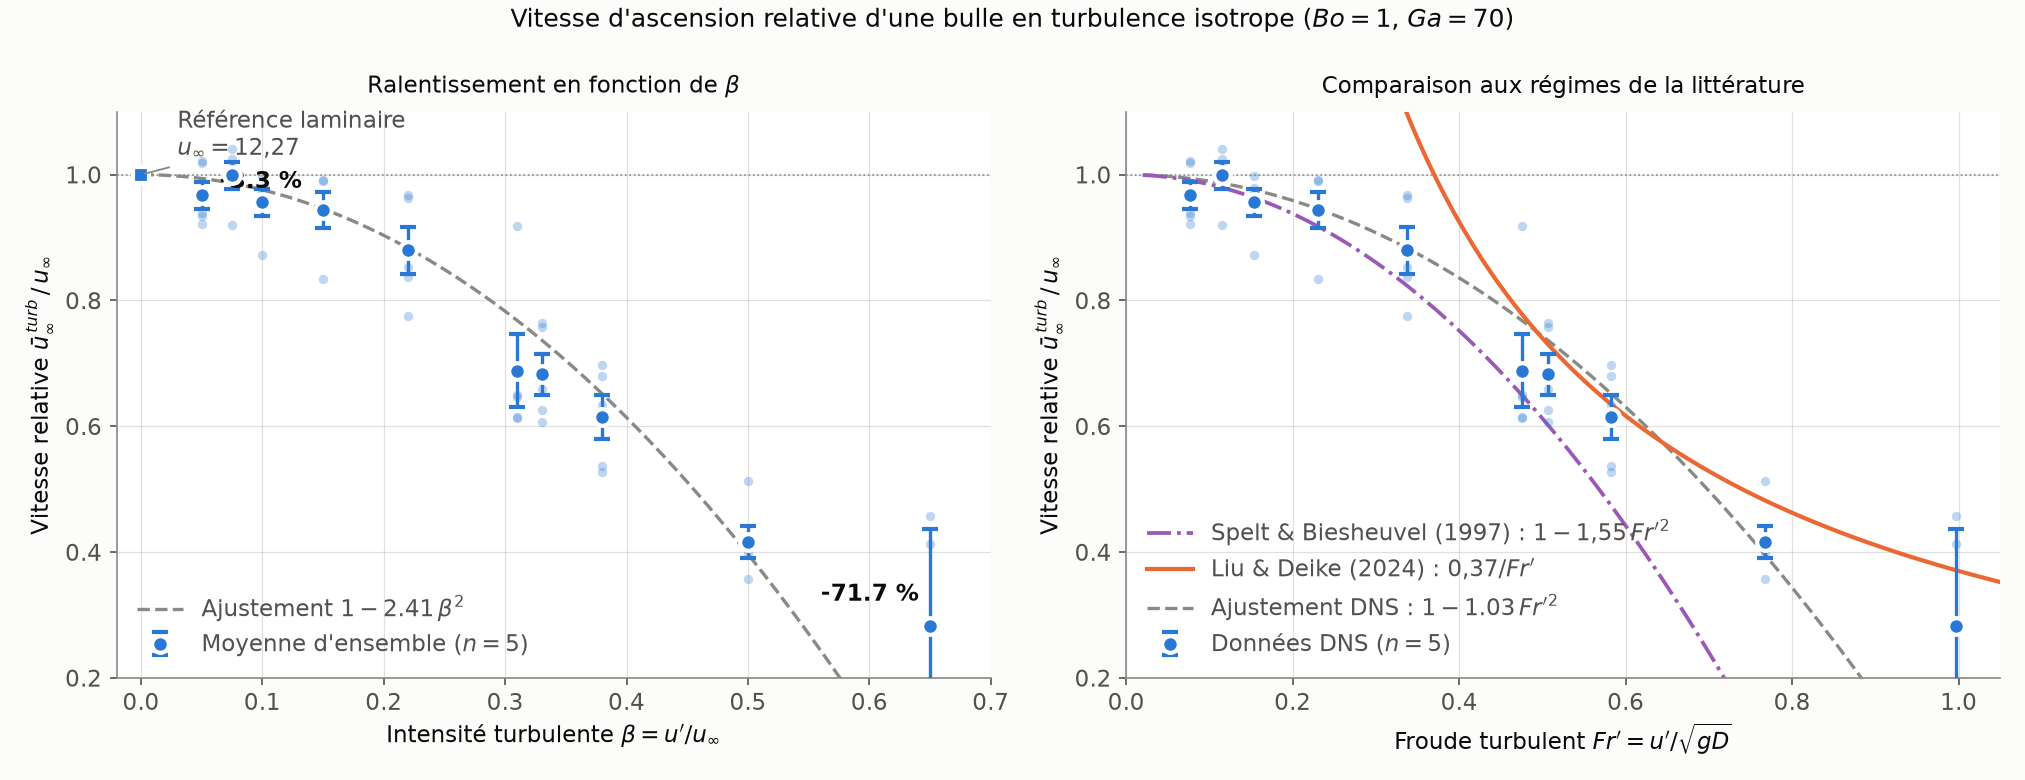
\includegraphics[width=0.88\textwidth]{ralentissement_beta_froude.png}

  \begin{itemize}
    \item \textbf{La turbulence ralentit systématiquement la remontée} ($\bar{u}_{\infty,\text{turb}} < u_\infty$).
    \item Réduction de \textbf{$-3\%$} à $\beta=0{,}05$ jusqu'à \textbf{$-72\%$} à $\beta=0{,}65$ ($n=5$ réalisations/point).
    \item Accord remarquable \textbf{sans aucun ajustement} avec la courbe de référence de la littérature (Liu \& Deike 2024).
  \end{itemize}
\end{frame}

% 5. Confrontation à la Littérature
\begin{frame}{Confrontation aux Deux Régimes de la Littérature}
  \begin{columns}[T]
    \begin{column}{0.5\textwidth}
      \begin{block}{Régime à faible Froude ($Fr' \lesssim 0{,}4$) -- Spelt \& Biesheuvel}
        $$\frac{\bar{u}_{\infty,\text{turb}}}{u_\infty} = 1 - c\,\beta^2 \quad (c \approx 2{,}41)$$
        \begin{itemize}
          \item Les points $\beta \in [0{,}05 \,;\, 0{,}15]$ confirment le comportement quadratique à l'origine.
        \end{itemize}
      \end{block}
    \end{column}

    \begin{column}{0.5\textwidth}
      \begin{block}{Régime à fort Froude ($Fr' \ge 0{,}5$) -- Liu \& Deike (2024)}
        $$\frac{\bar{u}_{\infty,\text{turb}}}{u_\infty} = \frac{0{,}37}{Fr'} \quad \left(Fr' = \frac{u'}{\sqrt{gD}}\right)$$
        \begin{itemize}
          \item À $\beta=0{,}50$ ($Fr'=0{,}77$) : DNS $= 0{,}416$ vs $0{,}37/Fr' = 0{,}482$.
          \item À $\beta=0{,}65$ ($Fr'=1{,}00$) : DNS $= 0{,}283$ vs $0{,}37/Fr' = 0{,}371$.
        \end{itemize}
      \end{block}
    \end{column}
  \end{columns}
\end{frame}

% 6. Mécanisme du Ralentissement
\begin{frame}{Identification du Mécanisme Physique}
  \begin{columns}[T]
    \begin{column}{0.52\textwidth}
      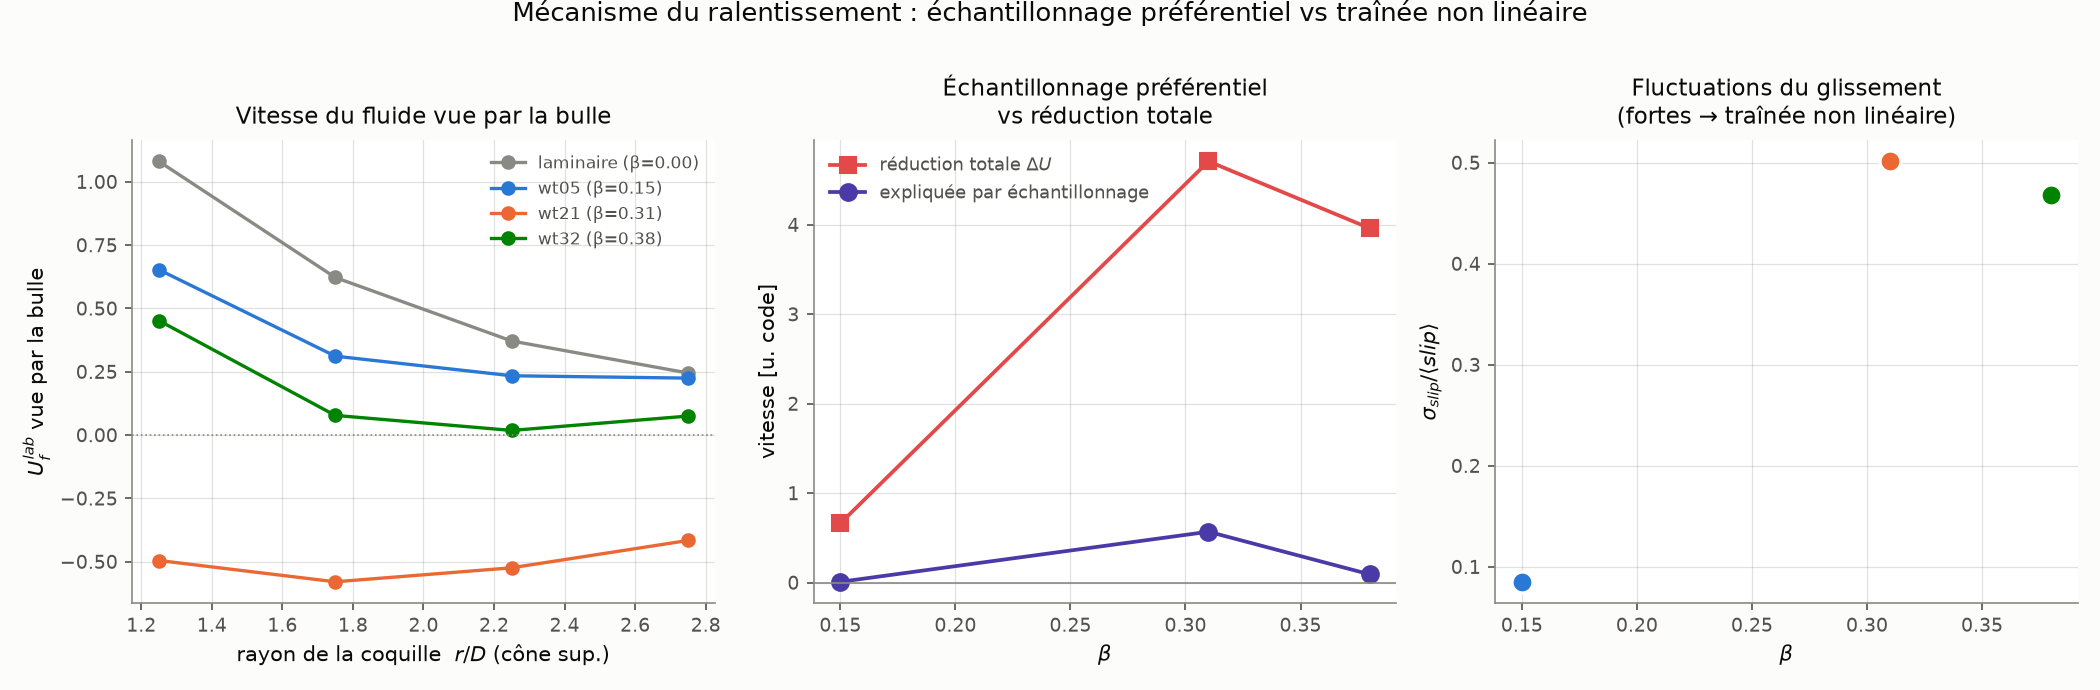
\includegraphics[width=\textwidth]{mechanism.png}
    \end{column}
    \begin{column}{0.45\textwidth}
      \begin{block}{Échantillonnage préférentiel vs Traînée non linéaire}
        \begin{itemize}
          \item \textbf{Échantillonnage préférentiel} : Vitesse du fluide vue par la bulle $\approx 0$ ($\le 12\%$ de la réduction).
          \item \textbf{Traînée non linéaire} : Les fluctuations de vitesse de glissement croissent de $8\%$ à $50\%$ avec $\beta$.
        \end{itemize}
      \end{block}
      \begin{alertblock}{Conclusion Mécanisme}
        Le ralentissement est \textbf{dominé par la traînée non linéaire} pour cette bulle super-Kolmogorov ($St \gg 1$).
      \end{alertblock}
    \end{column}
  \end{columns}
\end{frame}

% 7. Couverture de la Campagne & Non-Fragmentation
\begin{frame}{Couverture de la Campagne \& Intégrité de la Bulle}
  \begin{columns}[T]
    \begin{column}{0.55\textwidth}
      \centering
      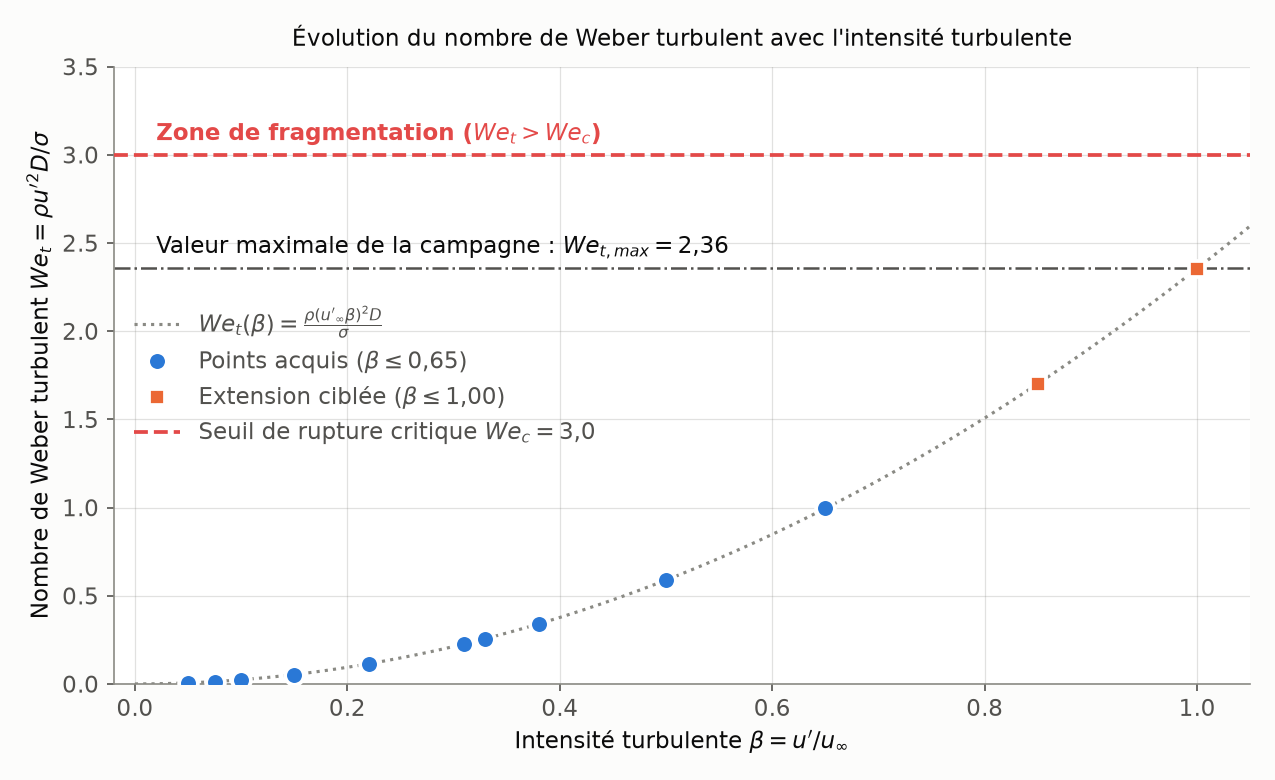
\includegraphics[width=\textwidth]{weber_turbulent_points.png}
    \end{column}
    \begin{column}{0.42\textwidth}
      \begin{block}{Sécurité vis-à-vis de la fragmentation}
        \begin{itemize}
          \item Campagne menée à $g=4 \implies \sigma = 1023$ (4$\times$ plus fort qu'à $g=1$).
          \item Le Weber turbulent $We_t = \frac{\rho u'^2 D}{\sigma}$ sature à $We_{t,\max} = 1{,}00 \le 3{,}0$.
          \item \textbf{Aucune rupture observée} sur les 10 points acquis : la bulle reste intacte et unique.
        \end{itemize}
      \end{block}
    \end{column}
  \end{columns}
\end{frame}

% 8. Bilan de la Campagne Numérique
\begin{frame}{Bilan Synthétique des 10 Points Acquis}
  \scriptsize
  \centering
  \renewcommand{\arraystretch}{1.2}
  \setlength{\tabcolsep}{3.5pt}
  \begin{tabular}{lcccccccccc}
    \toprule
    \textbf{Point} & \textbf{lo050} & \textbf{lo075} & \textbf{lo100} & \textbf{wt05} & \textbf{wt11} & \textbf{wt21} & \textbf{wt25} & \textbf{wt32} & \textbf{hi050} & \textbf{hi065} \\
    \midrule
    $\beta = u'/u_\infty$ & $0{,}05$ & $0{,}075$ & $0{,}10$ & $0{,}15$ & $0{,}22$ & $0{,}31$ & $0{,}33$ & $0{,}38$ & $0{,}50$ & $0{,}65$ \\
    $Fr' = u'/\sqrt{gD}$ & $0{,}077$ & $0{,}115$ & $0{,}153$ & $0{,}230$ & $0{,}337$ & $0{,}475$ & $0{,}506$ & $0{,}583$ & $0{,}767$ & $0{,}997$ \\
    $\bar{u}_{\infty,\text{turb}}$ & $11{,}86$ & $12{,}26$ & $11{,}73$ & $11{,}57$ & $10{,}79$ & $8{,}45$ & $8{,}38$ & $7{,}55$ & $5{,}11$ & $3{,}47$ \\
    $\bar{u}_{\infty,\text{turb}}/u_\infty$ & $0{,}97$ & $1{,}00$ & $0{,}96$ & $0{,}94$ & $0{,}88$ & $0{,}69$ & $0{,}68$ & $0{,}62$ & $0{,}42$ & $0{,}28$ \\
    \textbf{Réduction} & \textbf{$-3\%$} & \textbf{$0\%$} & \textbf{$-4\%$} & \textbf{$-6\%$} & \textbf{$-12\%$} & \textbf{$-31\%$} & \textbf{$-32\%$} & \textbf{$-38\%$} & \textbf{$-58\%$} & \textbf{$-72\%$} \\
    \bottomrule
  \end{tabular}

  \vspace{0.3cm}
  \textit{Chaque point correspond à la moyenne d'ensemble de $n=5$ réalisations turbulentes indépendantes.}
\end{frame}

% 9. Conclusion & Perspectives
\begin{frame}{Conclusion et Perspectives}
  \begin{columns}[T]
    \begin{column}{0.48\textwidth}
      \begin{block}{Conclusions principales}
        \begin{enumerate}
          \item La turbulence ralentit de manière monotone la vitesse d'ascension (jusqu'à $-72\%$).
          \item Validation complète de la courbe de référence ($1-c\beta^2 \to 0{,}37/Fr'$).
          \item Le ralentissement provient de la \textbf{traînée non linéaire}.
          \item Validation rigoureuse de la chaîne numérique sous Basilisk.
        \end{enumerate}
      \end{block}
    \end{column}

    \begin{column}{0.48\textwidth}
      \begin{block}{Perspectives directes}
        \begin{itemize}
          \item Récupérer les deux derniers points ultimes $\beta=0{,}85$ et $\beta=1{,}00$ (en cours sur Kairos).
          \item Varier le nombre de Bond $Bo$ à $Ga$ fixé pour tester l'effet de la déformabilité.
          \item Découpler l'intensité turbulente $\beta$ du Reynolds de maille $Re_\lambda$.
        \end{itemize}
      \end{block}
    \end{column}
  \end{columns}
\end{frame}

\end{document}
